\documentclass[xcolor=dvipsnames,aspectratio=1610]{beamer}
\usepackage{graphicx}
\usetheme[numbering=counter, progressbar=frametitle, sectionpage=none]{metropolis}
\title{Software Containers\ \

\includegraphics[scale=0.1]{whale.png}
\ 
\includegraphics[scale=0.15]{octopus.png}
\ 
\includegraphics[scale=0.1]{whale.png}}
\date{December 5, 2016}
\author{Shawn Seymour, Dan Stelljes}
\setbeamercolor{title separator}{fg=Cyan!60}
\setbeamercolor{progress bar}{fg=NavyBlue}
\setbeamercolor{frametitle}{fg=Black,bg=Cyan!60}
\setbeamercolor{alerted text}{fg=BurntOrange}


\begin{document}
  \maketitle
  \begin{frame}{Virtual Machines vs. Containers}
      \alert{Virtual machines} act as hardware virtualization and run a full operating system as a guest.
      \begin{itemize}
          \item Can be several gigabytes in size and take awhile to start up.
      \end{itemize}
      \vspace{10px}

      \alert{Containers} act as operating system virtualization where they share the kernel of the host machine.
      \begin{itemize}
          \item Can be tens of megabytes and start up instantly.
      \end{itemize}

  \end{frame}

  \begin{frame}{Virtual Machines vs. Containers}
      \begin{figure}
        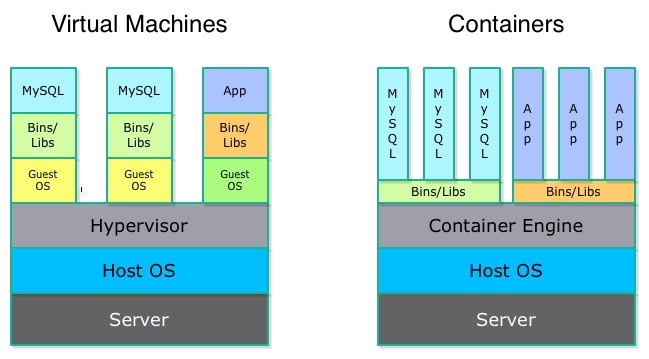
\includegraphics[scale=0.5]{container_vs_vm.jpg}
      \end{figure}
      Containers are used as a lightweight alternative to virtual machines and are very useful when deploying and running applications in clustered environments.

    \end{frame}


  \begin{frame}{Applications of Containers}
    So why containers?

    \begin{itemize}
        \item They can easily be spun up, worked with, destroyed, re-created, and built upon.
        \item Containers provide isolation; for example, in a web stack, the server and database can be hosted on the same machine but isolated in their own containers.
        \item It is very easy to scale applications over multiple containers as well as multiple hosts in a cluster setup.
    \end{itemize}

    \vspace{10px}

    Containers are typically used in one of two ways: to act as a full operating system or to run a single application. There are container environments made for each philosophy.
  \end{frame}

  \begin{frame}{Container Environments: For Systems}
      The following systems are meant to be used as a whole operating system: \newline
      \begin{itemize}
          \setlength\itemsep{1.6em}
          \item \alert{LXC} (\textbf{L}inu\textbf{X} \textbf{C}ontainers): One of the original container environments. Low-level, bare-bones container engine. Over eight years old.
          \item \alert{LXD}: An easier way to run LXC containers. Provides a wrapper over the low-level LXC interface.
      \end{itemize}
  \end{frame}

  \begin{frame}{Container Environments: For Applications}
      The following systems are meant to host single applications: \newline
      \begin{itemize}
          \setlength\itemsep{1.6em}
          \item \alert{Docker}: A platform for developing, shipping, and deploying single applications. Easy to setup and use. Currently the most common container environment.
          \item \alert{rkt}: The newest, cutting-edge container environment. Designed to address security issues with Docker and to standardize specifications for application containers.
      \end{itemize}
  \end{frame}

  \begin{frame}{Lab Suggestions}
      We did some cool things and proposed some ideas for the dungeon:
      \begin{itemize}
          \item \alert{Trac}, the lab's issue management system, can be hosted in a container rather than a virtual machine.
          \item \alert{Puppet}, the lab's configuration management tool, can also be hosted in a container.
          \item \alert{LDAP}, the lab's authentication manager, can be hosted in a single or multiple container setup. This allows for load balancing and faster logins.
          \item \alert{Distributed Research} could benefit from running research applications inside of containers across the cluster of lab machines.
      \end{itemize}
  \end{frame}

  \begin{frame}{Course Suggestions}
      Containers could be beneficial in multiple courses at UMM:
      \begin{itemize}
          \item \alert{Computing Systems: Practicum} (3403) could use LXD containers to blow up the world and mess around with networking without exposing the dungeon to the outside.
          \item \alert{Software Design} (3601) could use Docker containers for deployment of their web server and database. This allows for a live, isolated production environment.
      \end{itemize}
  \end{frame}

  \begin{frame}{Setup Diagram}
      \vspace{-30px}
      \begin{figure}
        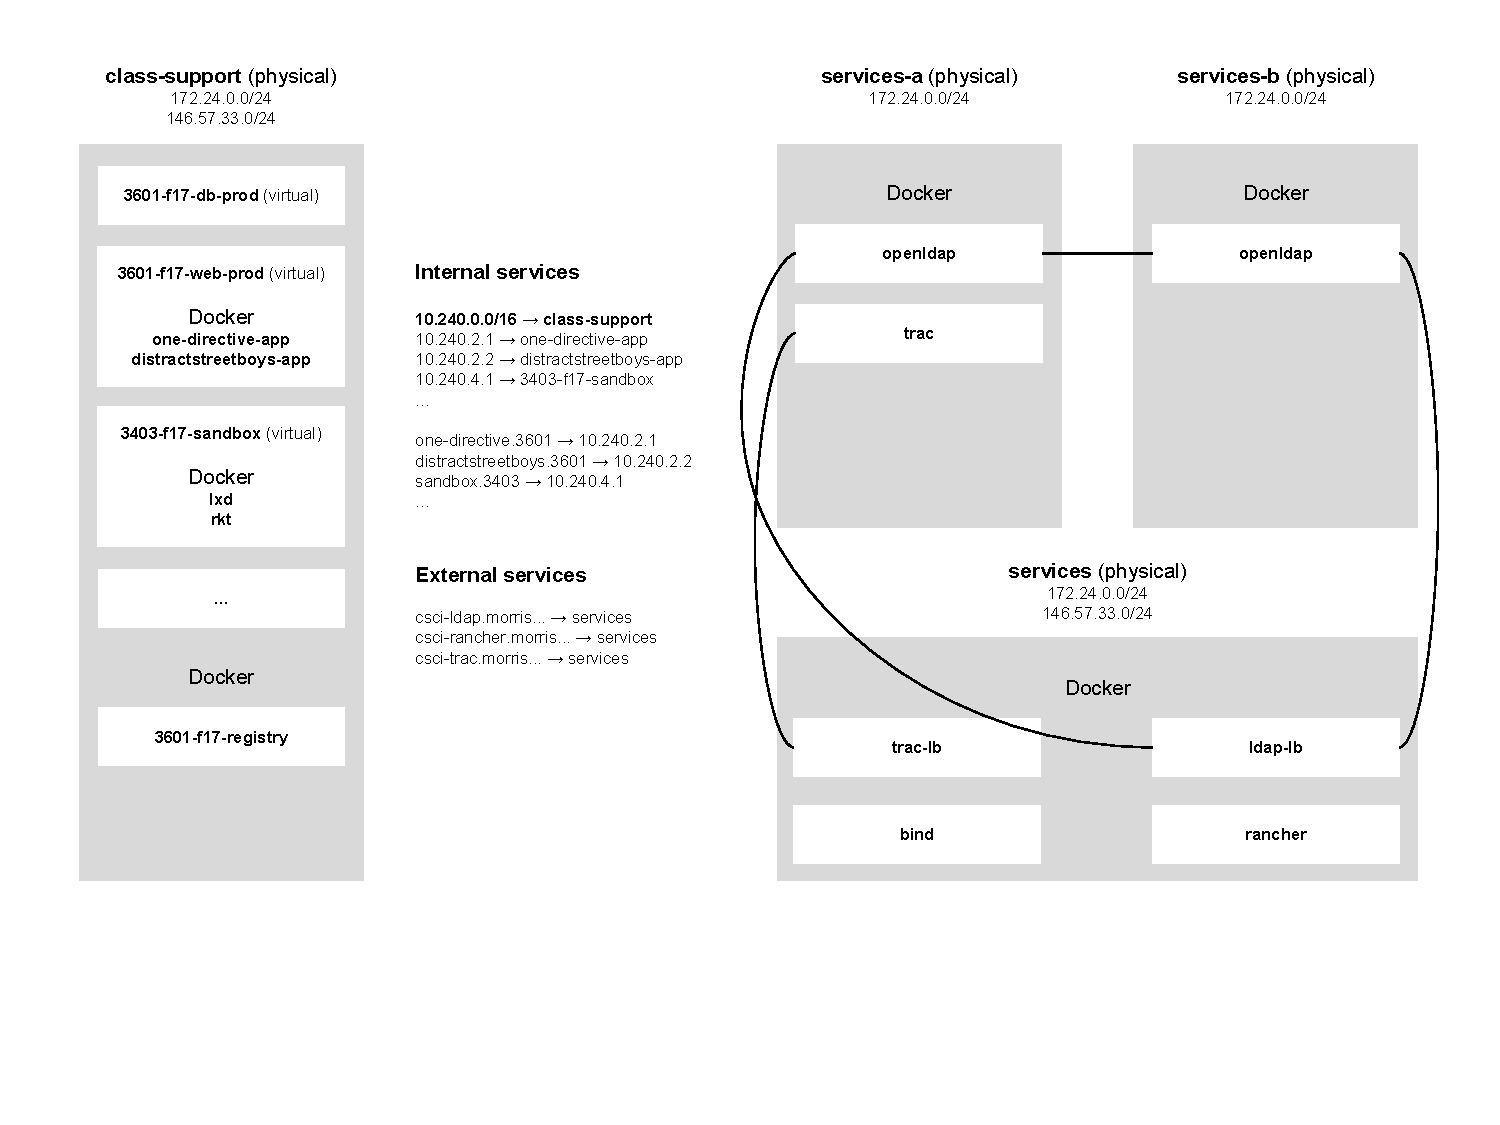
\includegraphics[scale=0.56]{proposal.pdf}
      \end{figure}
  \end{frame}

  \begin{frame}{Container Demos}
      We have a few demos of different software container applications to play around with: \newline
      \begin{itemize}
        \setlength\itemsep{1.6em}
        \item Dies Irae: Blow up the world challenge; example of LXD containers.
        \item Paula Deen's Thanksgiving: Nesting Docker inside of LXD.
        \item Down The Pipeline: Manipulating images by Docker and Rancher.
      \end{itemize}

  \end{frame}

  \begin{frame}{Appendix A: Kyle Hakala or Seth Meyers?}

      \begin{figure}
      \centering
      \begin{minipage}{.5\textwidth}
        \centering
        
\includegraphics[width=\linewidth]{kyle.png}
      \end{minipage}%
      \begin{minipage}{.5\textwidth}
        \centering
        
\includegraphics[width=.8\linewidth]{seth.jpg}
      \end{minipage}
      \end{figure}

  \end{frame}

  \begin{frame}{Appendix B}
      \begin{figure}
        
\includegraphics[scale=0.6]{cactus.png}
      \end{figure}
  \end{frame}

\end{document}
